%!TEX program = xelatex

%!TEX program = xelatex
% ****** Start of file TLGtheory.tex ******
%

\documentclass[%
 % reprint,
%superscriptaddress,
groupedaddress,
%unsortedaddress,
%runinaddress,
%frontmatterverbose, 
%preprint,
showpacs,
%preprintnumbers,
%nofootinbib,
%nobibnotes,
%bibnotes,
 amsmath,amssymb,
 aps,
%pra,
prb,
% rmp,
%prstab,
%prstper,
%floatfix,
]{revtex4-1}

\usepackage{graphicx}% Include figure files
\usepackage{dcolumn}% Align table columns on decimal point
\usepackage{bm}% bold math
\usepackage{hyperref}% add hypertext capabilities
\usepackage{braket}
\newcommand{\etal}{\textit{et.al}}

%\usepackage[mathlines]{lineno}% Enable numbering of text and display math
%\linenumbers\relax % Commence numbering lines

%\usepackage[showframe,%Uncomment any one of the following lines to test 
%scale=0.7, marginratio={1:1, 2:3}, ignoreall,% default settings
%text={7in,10in},centering,
%margin=1.5in,
%total={6.5in,8.75in}, top=1.2in, left=0.9in, includefoot,
%height=10in,a5paper,hmargin={3cm,0.8in},
%]{geometry}

% all eps files are in the figures 
% \graphicspath{{figures/}}

\begin{document}

\preprint{APS/123-QED}

\title{A brief introduction to superconducting qubits}% 
%\thanks{}%

% \input{authors}
\author{Wentao Jiang}%
 \email{jwt13@mails.tsinghua.edu.cn}
 \affiliation{%
Center for Quantum Information, IIIS, Tsinghua University, Beijing 100084, China
}%
 \affiliation{%
Department of Physics, Tsinghua University, Beijing 100084, China
}%

\date{\today}

\begin{abstract}
This is the Appendix A of my undergraduate thesis, a brief introduction to superconducting qubits (mainly about transmon qubits).
% To be added
%\begin{description}
%\item[PACS numbers]
%May be entered using the \verb+\pacs{#1}+ command. 
%\end{description}
\end{abstract}

% \pacs{71.70.Di,73.21.-b,73.21.La,73.22.Pr}% PACS, the Physics and Astronomy
                             % Classification Scheme.
%\keywords{Suggested keywords}%Use showkeys class option if keyword
                              %display desired
\maketitle

\tableofcontents
% \nocite{*}




This appendix is designed to be a concise introduction to superconducting qubits with a focus on transmon qubits, including the theoretic derivation of its Hamiltonian and properties, a brief history of the development of transmon qubits and crucial technical improvements. See, for example, Ref.~\onlinecite{Clarke2008,devoret2013superconducting,Wendin2016} for a more detailed review about superconducting qubits.

This appendix is written as a `router' for more detailed literature on topics included, with the most important results and conclusions explicitly presented here.

\section{Principle of superconducting qubits} % (fold)
\label{sec:principle_of_superconducting_qubit}
    
    When talking about a qubit, and more generally quantum information processing, the first thing is the criteria for a good qubit, which is originally proposed by DiVincenzo\cite{divincenzo2000physical} and is known as the DiVincenzo criteria
    \begin{enumerate}
        \item Qubits: fabrication of registers with several (many) qubits
        \item Initialization: the qubit register must be possible to initialise to a known state
        \item Universal gate operations: high fidelity single and 2-qubit gate operations available
        \item Readout: the state of the qubit register must be possible to read out, typically via readout of individual qubits
        \item Long decoherence times: large number of single and 2-qubit gate can be performed within the qubit decoherence time
        \item Quantum interfaces for qubit interconversion
        \item Quantum interfaces to flying qubits for optical communication
    \end{enumerate}
    I'll try to cover the above seven points for superconducting qubits.


    \subsection{Hamiltonian of Transmon} % (fold)
    \label{sub:hamiltonian_of_transmon}
    A superconducting qubits can be viewed as a superconducting nonlinear oscillator. For a simple linear oscillator, the Hamiltonian is
    \begin{equation}
    \label{eqn:linearOscillatorHam}
        H = 4E_C \hat n^2 + E_L \frac{\hat \delta^2}{2}
    \end{equation}
    where $\hat n$ is the excess charge on the capacitor in units of 2e and $ \hat \delta  $ is the phase difference of the inductor. $E_C = e^2/2C$ is the charging energy\cite{koch2007charge} and $E_L = \Phi_0^2/4 \pi^2 L $ is the energy of one flux quantum. You might see $\hat n - n_g$ instead of $\hat n$ in literature, where $\hat n$ is total charge operator and $n_g$ is the effective offset charge controlled by a capacitively coupled gate. Also in some literature, charging energy $E_C$ is defined as $ (2e)^2/2C $ so that there's no factor $4$ before the charge term of the Hamiltonian (see, e.g., Ref.~\onlinecite{Wendin2016,Collin2004}).

    This harmonic oscillator Hamiltonian leads to evenly spaced energy levels and can not be used as a qubit with effectively two levels. A nonlinear element called Josephson junction (J-J) is utilized to bring aharmonicity to the system. A J-J is realized by separating two superconducting regions with a thin insulator. The insulator is thin enough to allow the tunneling of Cooper pairs across the junction. The most important phenomena in a J-J is the current-phase and voltage-phase relation (see Appendix A of Ref.~\onlinecite{Raab2015} for a brief derivation):
    \begin{align}
    \label{eqn:currentVoltagePhase}
        I &= I_c \sin \delta \\
        \dot \delta & = \frac{2e}{\hbar} V = \frac{2 \pi}{\Phi_0} V
    \end{align}
    Where $ \delta $ is the phase difference across the junction. As a result, the energy of a J-J is\cite{Raab2015}
    \begin{equation}
        H_J = \int dt VI = \frac{\Phi_0 I_c}{2 \pi}\int dt \dot \delta \sin \delta = -\frac{\Phi_0 I_c}{2 \pi}\cos \delta = -E_J \cos \delta
    \end{equation}
    Hence when using a J-J as an nonlinear inductance, the Hamiltonian (\ref{eqn:linearOscillatorHam}) becomes
    \begin{equation}
        H = 4E_C \hat n^2 -E_J \cos \hat \delta  
    \end{equation}

    The exact solution of the energy levels of the above Hamiltonian includes Mathieu functions\cite{schuster2007circuit,koch2007charge}. For transmon qubits with $E_J /E_C \sim 100$, the energy levels simplified to\cite{koch2007charge}
    \begin{equation}
    \label{eqn:transmonLevels}
        E_m \approx -E_J + \sqrt{8E_CE_J} \left (m+\frac{1}{2} \right ) - \frac{E_C}{12}(6m^2+6m+3)
    \end{equation}
    where $ \omega_p = \sqrt{8E_CE_J}/\hbar   $ is known as the plasma frequency. Absolute and relative anharmonicity is often defined to characterize the transmon anharmonicity, which are
    \begin{align}
        \alpha &\equiv E_{12} - E_{01} \approx -E_C\\
        \alpha_r & \equiv \alpha/E_{01} \approx -(8E_J/E_C)^{-1/2}
    \end{align}
    
    In some superconducting qubit design, two J-J are used to form a SQUID. The Hamiltonian of a SQUID is\cite{koch2007charge}
    \begin{equation}
        H_J = -E_{J1}\cos \delta_1 -E_{J2}\cos \delta_2
    \end{equation}
    where $ \delta_{1,2} $ now describe the phase difference across the junctions. Flux quantization then require (see Appendix A of Ref.~\onlinecite{Raab2015} for a simple derivation)
    \begin{equation}
        \delta_1 - \delta_2 = 2 \pi n + 2 \pi \Phi/\Phi_0
    \end{equation}
    where $n$ is an integer, $\Phi $ is the flux through the SQUID ring which is adjustible by, e.g.,  a nearby wire, and $ \Phi_0 =h/2e  $ is the superconducting flux quantum. Define the effective phase difference $ \delta = (\delta_1+\delta_2)/2 $, $E_{J \Sigma} = E_{J1} + E_{J2} $ and the junction asymmetry $d = (E_{J2}- E_{J1})/(E_{J2}+E_{J1}) $ which is typically 10\%, the SQUID Hamiltonian can be written as\cite{koch2007charge}
    \begin{equation}
        H_J = - E_{J \Sigma} \cos \left (\frac{\pi \Phi}{\Phi_0} \right )\sqrt{ 1+d^2 \tan^2 \left (\frac{\pi \Phi}{\Phi_0} \right ) }\cos(\hat \delta - \delta_0)
    \end{equation}
    where $ \delta_0 $ determined by $ \tan \delta_0 = d \tan(\pi \Phi/\Phi_0) $. The presence of $ \delta_0 $ in SQUID with asymmetric junctions can lead to additional qubit control and hence additional decay channel. As a result, using a symmetric SQUID instead of a simple J-J gives rise to qubits with tunable junction energy $ E_J = E_{J \Sigma} \cos(\pi \Phi/\Phi_0) $.

        
    % subsection hamiltonian_of_transmon_and_transmon_in_cqed (end)
    

    \subsection{Control and readout of transmon qubits} % (fold)
    \label{sub:control_and_readout_of_transmon_qubits}

        A schematic figure of transmon circuit is shown in Fig.~\ref{fig:transmonSchematic}.

            \begin{figure}[h]
                \centering
                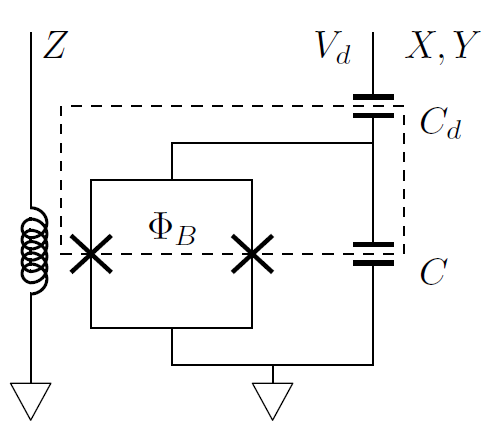
\includegraphics[width=3in]{transmon_scheme.png}
                \caption{Transmon circuit with X, Y and Z control, adapted from Ref.~\onlinecite{Raab2015}.}
                \label{fig:transmonSchematic}
            \end{figure}
            Where the drive voltage $V_d$ can come from both a microwave cavity field\cite{koch2007charge} and an independent drive line\cite{Barends2013Coherent}. The X control is realized by flux-biasing the SQUID, temporarily changing the transmon energy spacing according to eqn.~(\ref{eqn:transmonLevels}). Following Ref.~\onlinecite{Raab2015}, the Hamiltonian of the transmon with drive $ V_d $ is
            \begin{equation}
            \label{eqn:transmonWithDrive}
                H = 4E_C \hat n^2  - E_J \cos \delta + \frac{C_d}{C_\Sigma} 2eV_d \hat n
            \end{equation}
            where the charge operator $\hat Q$ in Ref.~\onlinecite{Raab2015} is substituted to $ 2e \hat n $. Eqn.~(\ref{eqn:transmonWithDrive}) is comparable to Eqn.~(3.1) in Ref.~\onlinecite{koch2007charge}, which I also include here:
            \begin{equation}
            \label{eqn:transmonWithCavityDrive}
                H = 4E_C (\hat n - n_g)^2 - E_J \cos \delta +2 \beta e V^0_{\text{rms}}\hat n( \hat a + \hat a^\dagger ) + \hbar \omega \hat a^\dagger \hat a
            \end{equation}
            where $n_g$ is the charge offset neglected in eqn.~(\ref{eqn:transmonWithDrive}). $ \beta = C_d/C_\Sigma $ is the ratio between the gate capacitance and the total capacitance. $V^0_{\text{rms}} $ is the zero-field root-mean-square voltage, hence $V^0_{\text{rms}}( \hat a + \hat a^\dagger ) = V_d$. The extra term $H_r = \hbar \omega \hat a^\dagger \hat a$ comes from the microwave resonator the transmon coupled to, which in not taken into account in Fig.~\ref{fig:transmonSchematic}.

            Expanding the Hamiltonian in transmon basis $ \ket{i} $, the Hamiltonian becomes
            \begin{align}
            \label{eqn:transmonWithCavityDriveExpanded}
                H &= \hbar \sum_j \omega_j \ket j \bra j + \hbar \omega_r \hat a^\dagger \hat a + \hbar \sum_{i,j} g_{ij} \ket i \bra j (\hat a + \hat a^\dagger ) \\
                \label{eqn:simplifiedTransmonWithCavityDrive}
                & \approx \hbar \sum_j \omega_j \ket j \bra j + \hbar \omega_r \hat a^\dagger \hat a  + \left (\hbar \sum_{i} g_{i,i+1} \ket i \bra{i+1} \hat a^\dagger + h.c. \right )
            \end{align}
            where $\hbar g_{ij} = 2 \beta e V^0_{\text{rms}} \bra i \hat n \ket j$. The approximation $ |\bra{j+k}\hat n \ket j| \rightarrow 0  $ when $|k|>1, E_J/E_C \rightarrow \infty $ and rotating wave approximation (RWA) are adopted. The non-vanishing coupling matrix elements are
            \begin{equation}
            \label{eqn:couplingElements}
                | \bra{j+1} \hat n \ket j |\approx \sqrt{ \frac{j+1}{2}} \left ( \frac{E_J}{8E_C} \right )^{1/4} 
            \end{equation}

            When the state space is further restricted to the ground and first excite state, the Hamiltonian (\ref{eqn:simplifiedTransmonWithCavityDrive}) reduce to the Jaynes-Cummings Hamiltonian\cite{walls2007quantum,schuster2007circuit}
            \begin{equation}
            \label{eqn:JCHamiltonian}
                H = \hbar \frac{\omega_{01}}{2} \hat \sigma_z + \hbar \omega_r \hat a^\dagger \hat a  + \hbar (g_{01}\hat a^\dagger \hat \sigma^- + h.c. )
            \end{equation}
            where $ \hbar \omega_{01} = \sqrt{8E_JE_C} - E_C $ is the qubit energy separation.
            
            If we start from eqn.~(\ref{eqn:simplifiedTransmonWithCavityDrive}) but without the RWA, switch back to classical drive field $V_d = V_{d0}\cos(\omega_d t + \phi) $ without the cavity and keep only the lowest two levels, the Hamiltonian turns to
            \begin{align}
                H &= \hbar \frac{\omega_{01}}{2} \hat \sigma_z + 2 \beta e \sqrt{ \frac{1}{2}} \left ( \frac{E_J}{8E_C} \right )^{1/4} V_{d0} \hat \sigma_x \cos(\omega_d t + \phi) \\
                &=   \hbar \frac{\omega_{01}}{2} \hat \sigma_z + \Omega \hat \sigma_x \cos(\omega_d t + \phi)
            \end{align}
            Transforming into the rotating frame with the drive frequency by applying $ U = \exp(i \omega_d t \hat \sigma_z /2) $ such that $ H_{RF} = UHU^\dagger + i\hbar \dot U U^\dagger $, the Hamiltonian becomes
            \begin{align}
                H_{RF} &= \hbar \frac{\omega_{01} - \omega_d}{2} \hat \sigma_z + \Omega ( \cos (\omega_d t) \hat \sigma_x - \sin (\omega_d t) \hat \sigma_y )\cos(\omega_d t + \phi)\\
                & = \hbar \frac{\omega_{01} - \omega_d}{2} \hat \sigma_z + \frac{\Omega}{2} \cos \phi \hat \sigma_x+ \frac{\Omega}{2} \sin \phi \hat \sigma_y
            \end{align}
            where the terms rotating at $ 2 \omega_d t $ is thrown away by RWA. The resulting Hamiltonian shows that the drive effectively rotate the qubit state along the axis $B_{\text{eff}} = ((\omega_{01} - \omega_d)/2,\Omega \cos \phi /2,\Omega \sin \phi /2)$, like a spin-1/2 particle in the effective magnetic field $B_{\text{eff}}$, realizing the X and Y drive.

            In most circumstances, a transmon qubit is coupled to a microwave resonator for readout, and the corresponded Hamiltonian is identical to eqn.~(\ref{eqn:JCHamiltonian}). When the resonator and transmon are detuned from each other, the J-C Hamoltonian goes to the dispersive limit\cite{Blais2004,schuster2007circuit}
            \begin{equation}
                H \approx \hbar \left (\omega_r + \frac{g_{01}^2}{\Delta} \hat \sigma_z \right )\hat a^\dagger \hat a+ \frac{1}{2} \hbar \left(\omega_{01} + \frac{g_{01}^2}{\Delta}\right) \hat \sigma_z
            \end{equation}
            where $ \Delta = \omega_{01} - \omega_r \gg g_{01}$ is the transmon-cavity detuning. Explicitly, the cavity resonant frequency depends on the state of the transmon, hence by probing the cavity response, the state of the transmon can be extracted. Single-shot readout can be achieved by proper amplification process\cite{Mallet2009,Sliwa2016}.


        
    % subsection control_and_readout_of_transmon_qubits (end)

    \subsection{Decay and dephasing in transmon qubits} % (fold)
    \label{sub:decay_and_dephasing_in_transmon_qubits}

    Decay and dephasing are both large topics and won't be covered here for detail.

    Chapter 4 in Ref.~\onlinecite{schuster2007circuit} theoretically discussed decoherence in superconducting qubits in great detail, including voltage noises, material loss, dipole radiation, charge and flux noise and $E_J$ and $E_C$ noise. Transmon was proposed to fight against charge noise.

    Ref.~\onlinecite{Martinis2014Report} discussed decoherence in transmon qubit experimentally. Capacitor loss, inductor and junction loss, and radiation and wiring loss were discussed. Many technical details are involved to obtain qubits with higher coherence and these details will be mentioned in \ref{sec:technical_improvements}.
    
    % subsection decay_and_dephasing_in_transmon_qubits (end)
    

% section principle_of_superconducting_qubit (end)


\section{A brief history of the development of transmon qubits} % (fold)
\label{sec:history_of_the_development_of_transmon_qubit}

The superconducting qubits evolves from Cooper pair box (CPB), which is basically a charge island separated from a charge reservoir by a J-J. Early research about CBP (originally called superconducting single-electron box\cite{Nakamura1997}) mainly concerned about its transport properties and charging effects. In 1999, superconducting flux qubit was proposed by Mooji \etal{}\cite{Mooij1999}, pulse modulation of quantum states were realized by Nakamura \etal\cite{Nakamura1999}. A gate voltage pulse brought two levels of the CPB into resonance and coherent oscillations in state population was observed by varying the pulse length. The coherence time was $\sim 1$ns. To obtain better coherence, the same group used spin-echo-type technique on the same system and identified the dominant dephasing source was the $1/f$ charge noise\cite{Nakamura2002}. More works quickly followed on similar system, with microwave pulses manipulating the qubit state\cite{Vion2002,Collin2004} and also with more complex device such as two coupled charge qubit\cite{Pashkin2003}. Ref.~\onlinecite{Makhlin2001} is a review about early but also fundamental superconducting qubit design.


            \begin{figure}[h]
                \centering
                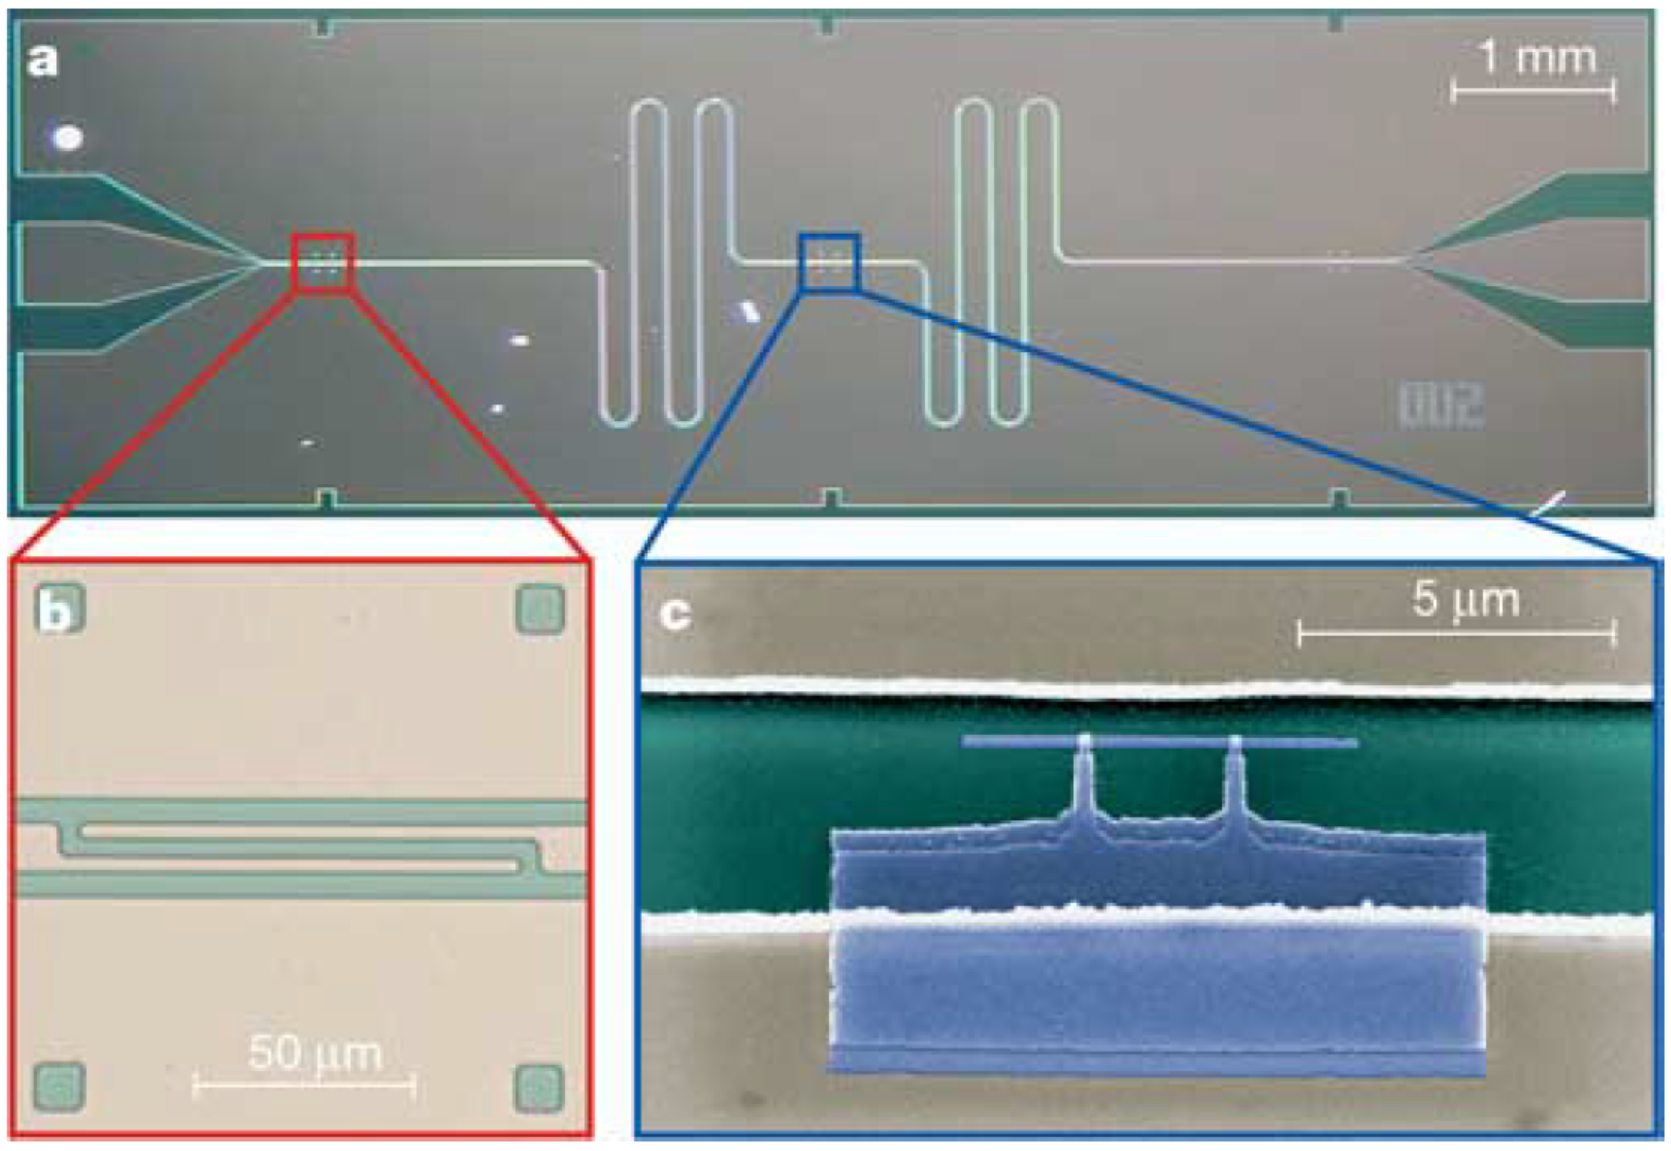
\includegraphics[width=4in]{review/strongCoupling2004.png}
                \caption{Strong coupling between superconducting qubit and single photon, adapted from Ref.~\onlinecite{Wallraff2004Nature}.}
                \label{fig:strongCoupling2004}
            \end{figure}

In 2004, Yale group proposed circuit quantum electrodynamics (cQED) as an architecture for quantum computation, where superconducting qubits are coupled to CPW resonator for control and readout\cite{Blais2004}. In the same year, strong coupling between superconducting charge qubit and CPW resonator was achieved\cite{Wallraff2004Nature}. By probing the cavity transmission while manipulating the qubit level structure via gate voltage and flux bias, level structure and vacuum Rabi splitting were clearly observed. In their following experiments, effect of the ac Stark shift from the cavity on the qubit and hence the dephase from the photon shot noise is experimentally explored\cite{Schuster2005} and theoretically explained\cite{Gambetta2006}. The qubit line shape fits better to a Lorentzian (Gaussian) for low (high) intra-cavity photon number, which agrees with their theory of measurement-induced dephasing. The dephasing time exceeded 200ns in this work.


In 2007, The same group at Yale proposed more detailed single and two qubit(s) gate design for quantum information processing based on cQED\cite{Blais2007}. At the same time, coupling between remote qubits were realized with both phase qubits\cite{Sillanpaa2007} and charge qubits\cite{Majer2007} via a cavity bus. While probing the cavity resonance can be used for qubit readout, Schuster \etal{} showed that the qubit spectroscopy can be used to resolve photon number states of the cavity\cite{Schuster2007Resolving}.


            \begin{figure}[h]
                \centering
                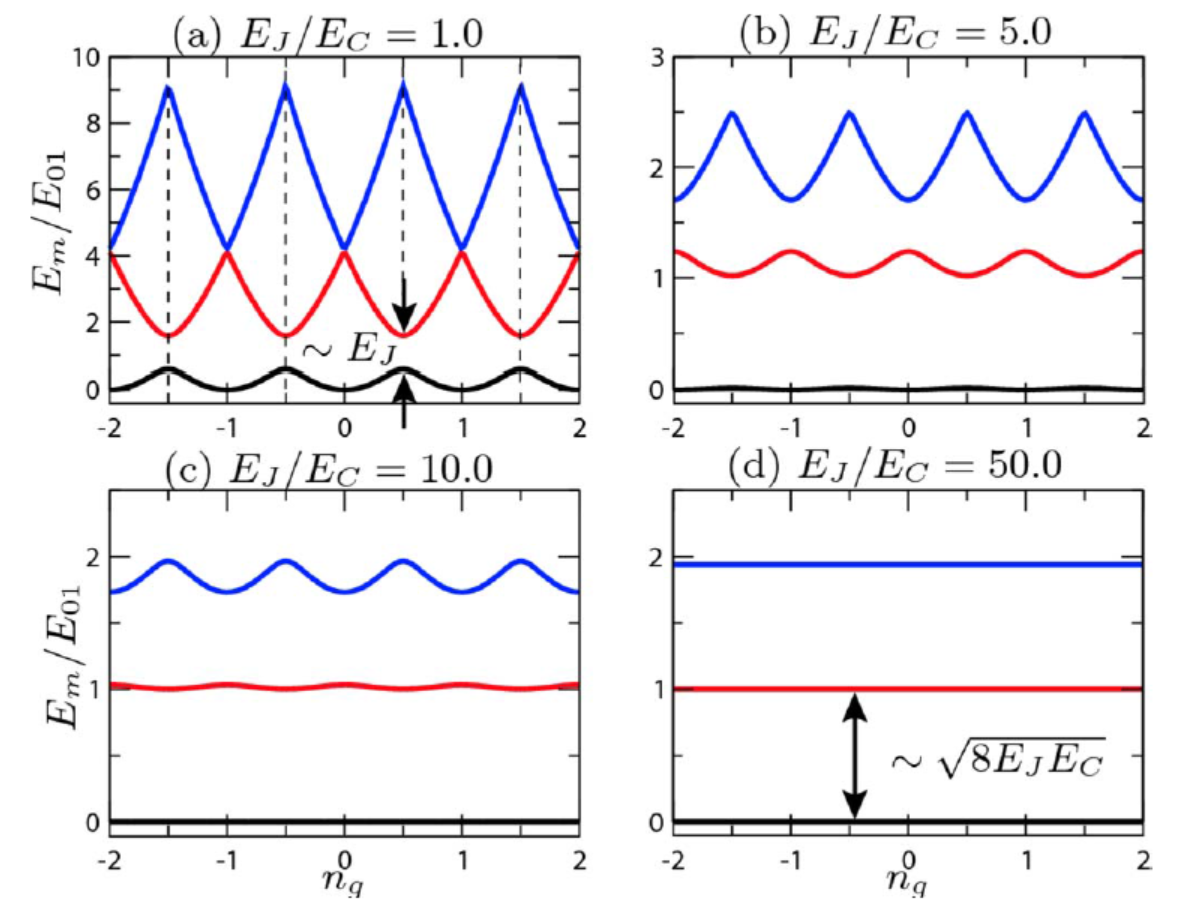
\includegraphics[width=4in]{review/transmon2007.png}
                \caption{Energy levels of superconducting qubit versus gate charge, with different $E_J/E_C$ value. Adapted from Ref.~\onlinecite{koch2007charge}.}
                \label{fig:transmon2007}
            \end{figure}


The charge qubits suffer from $1/f$ charge noise, since the energy levels depends on the gate induced charge $n_g$. Degrees of control always correspond to channels of dephasing. In order to suppress the sensitivity to charge noise, Koch \etal{} proposed transmon qubits\cite{koch2007charge}. The ratio between $E_J$ and $E_C$ is increased to suppress the dependence of energy levels with respect to $n_g$, while the anharmonicity still remains sufficient for defining qubits. Their proposal was quickly implemented approximately one year later\cite{Schreier2008}, where the various decay and dephasing times are all above 1$\mu$s.


            \begin{figure}[h]
                \centering
                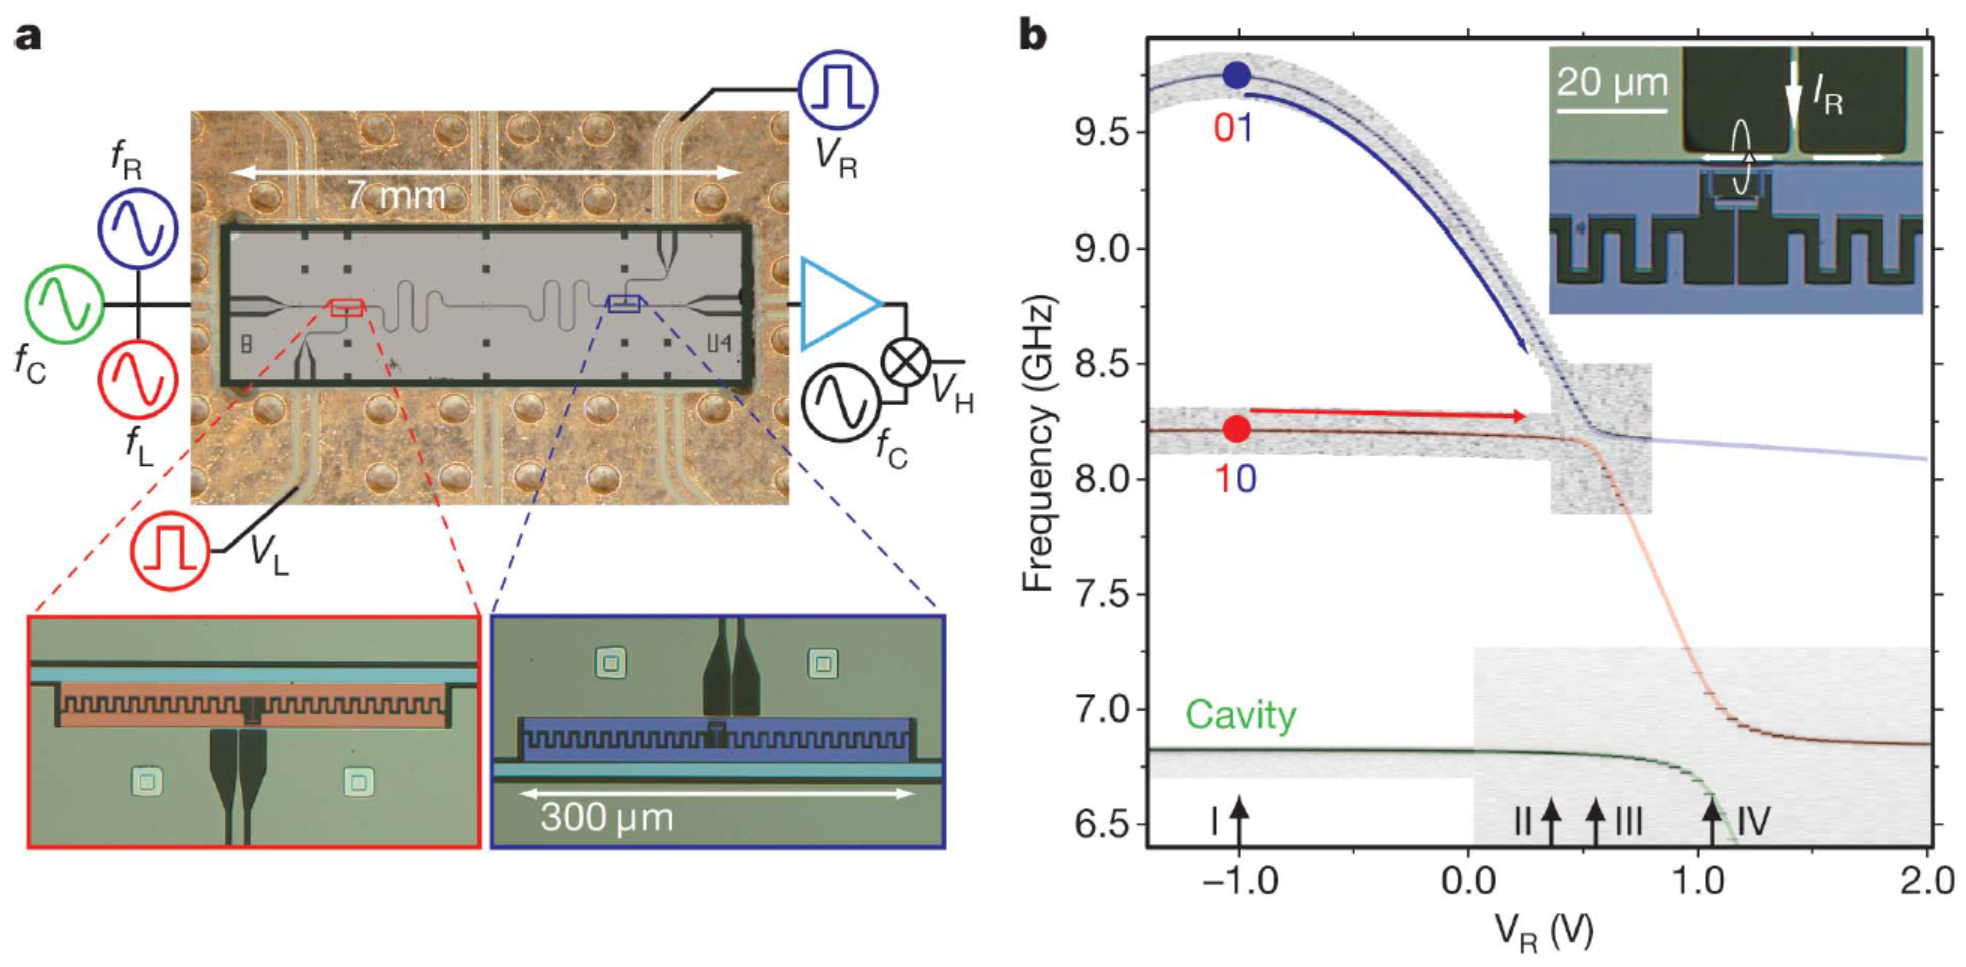
\includegraphics[width=5in]{review/twoQubit2009.png}
                \caption{Device for demonstration of two-qubit algorithms. Adapted from Ref.~\onlinecite{DiCarlo2009}.}
                \label{fig:twoQubit2009}
            \end{figure}

With the new transmon design and multiple qubit coupling, the Yale group soon proceeded to multi-qubit manipulations and readout. Two-qubit state tomography using a joint disppersive readout was proposed in Ref.~\onlinecite{Filipp2009}, where the cavity frequency shift depends on both states of the two qubits coupling to the cavity. With two transmons coupled to a cavity bus, DiCarlo \etal{} showed two-qubit algorithm in superconducting system\cite{DiCarlo2009}. Two qubit controlled phase gate was implemented utilizing level pulling from a non-computational state by adiabatic flux pulse. They soon went to couple four transmons in one cavity and succesfully prepared and measured a three-qubit entanglement\cite{DiCarlo2010}. The flux-pulse C-Phase gate was 12ns in their case and the qubit coherence time is on the level of $\sim 1 \mu$s.


            \begin{figure}[h]
                \centering
                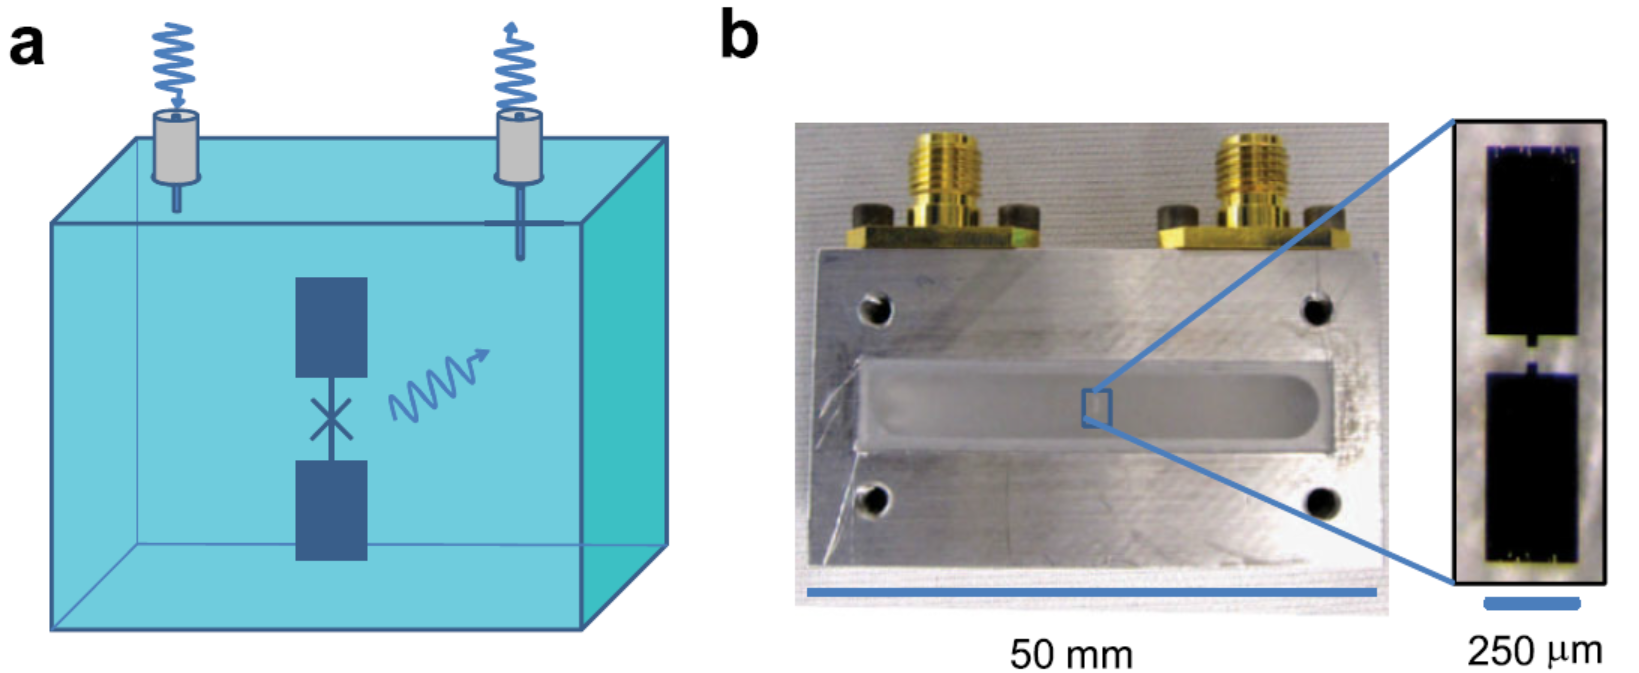
\includegraphics[width=4in]{review/3D_transmon2011.png}
                \caption{3D transmon design. Adapted from Ref.~\onlinecite{DiCarlo2009}.}
                \label{fig:Paik2011}
            \end{figure}

While the coherence time of superconducting qubits has been steadily improved from $\sim 1$ns in original CPB to $\sim 1 \mu$s for transmons, the Yale group made another drastic improvement by the 3D transmon design\cite{Paik2011}. The measured $T_1$ was up to $60\mu$s and $T_2 \sim 10\mu$s. The long coherence time benefitted from the avoidance of $1/f$ charge noise, single junction design and also material optimizations. The record and was soon further increased to $\sim 0.1$ms\cite{Rigetti2012} by reducing dephasing rate per residual cavity photon, minimize coupling to higher cavity mode and lowering the thermal photon temperature of the cavity.



            \begin{figure}[h]
                \centering
                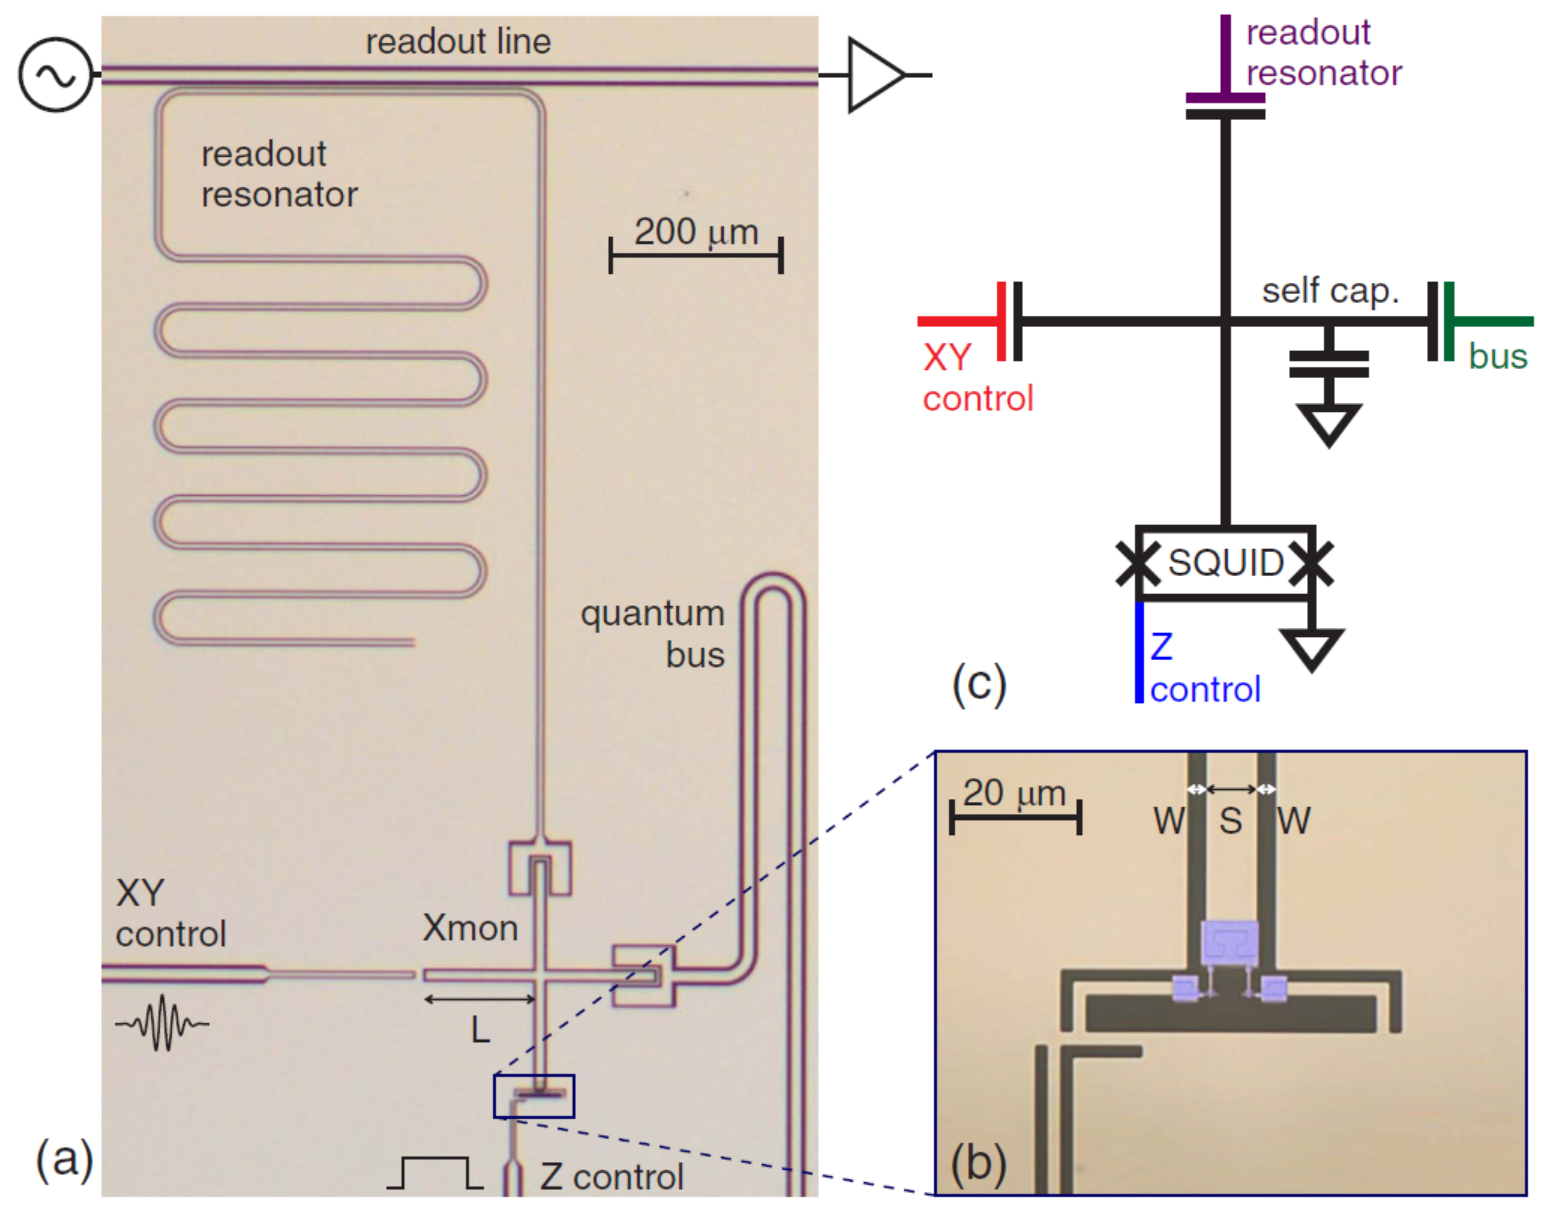
\includegraphics[width=4in]{review/XmonDesign2013.png}
                \caption{Xmon design. Adapted from Ref.~\onlinecite{Barends2013Coherent}.}
                \label{fig:XmonDesign2013}
            \end{figure}




Besides the Yale group, there are also many other groups working on superconducting qubits, in which Prof. Martinis' group at UCSB stands out. Beyond their previous interests in phase qubits, the UCSB group proposed a variation of transmon named Xmon\cite{Barends2013Coherent}, which was designed for scalability with surface code\cite{Fowler2012}. In the Xmon design, the resonator for qubit readout is modified from in-line reflection type to hanger type, allowing one transmission line to couple with many hanger resonators. The `X' shape of the qubit capacitor offers coupling to readout resonator, quantum bus, XY drive and Z control respectively. With a lot of technical improvements (see Sec.~\ref{sec:technical_improvements}), the Xmon qubit showed coherence time $\sim 15\mu$s. Based on the Xmon design, the same group at UCSB increased the number of coupled Xmon qubits to five\cite{Barends2014} and nine\cite{Kelly2015} in the year 2014 and 2015 respectively. These qubits have coherence time $\sim 30\mu$s, single qubit gates fidelity all above 0.999 and two-qubit gate fidelity above 0.99 between all coupled qubits.


            \begin{figure}[h]
                \centering
                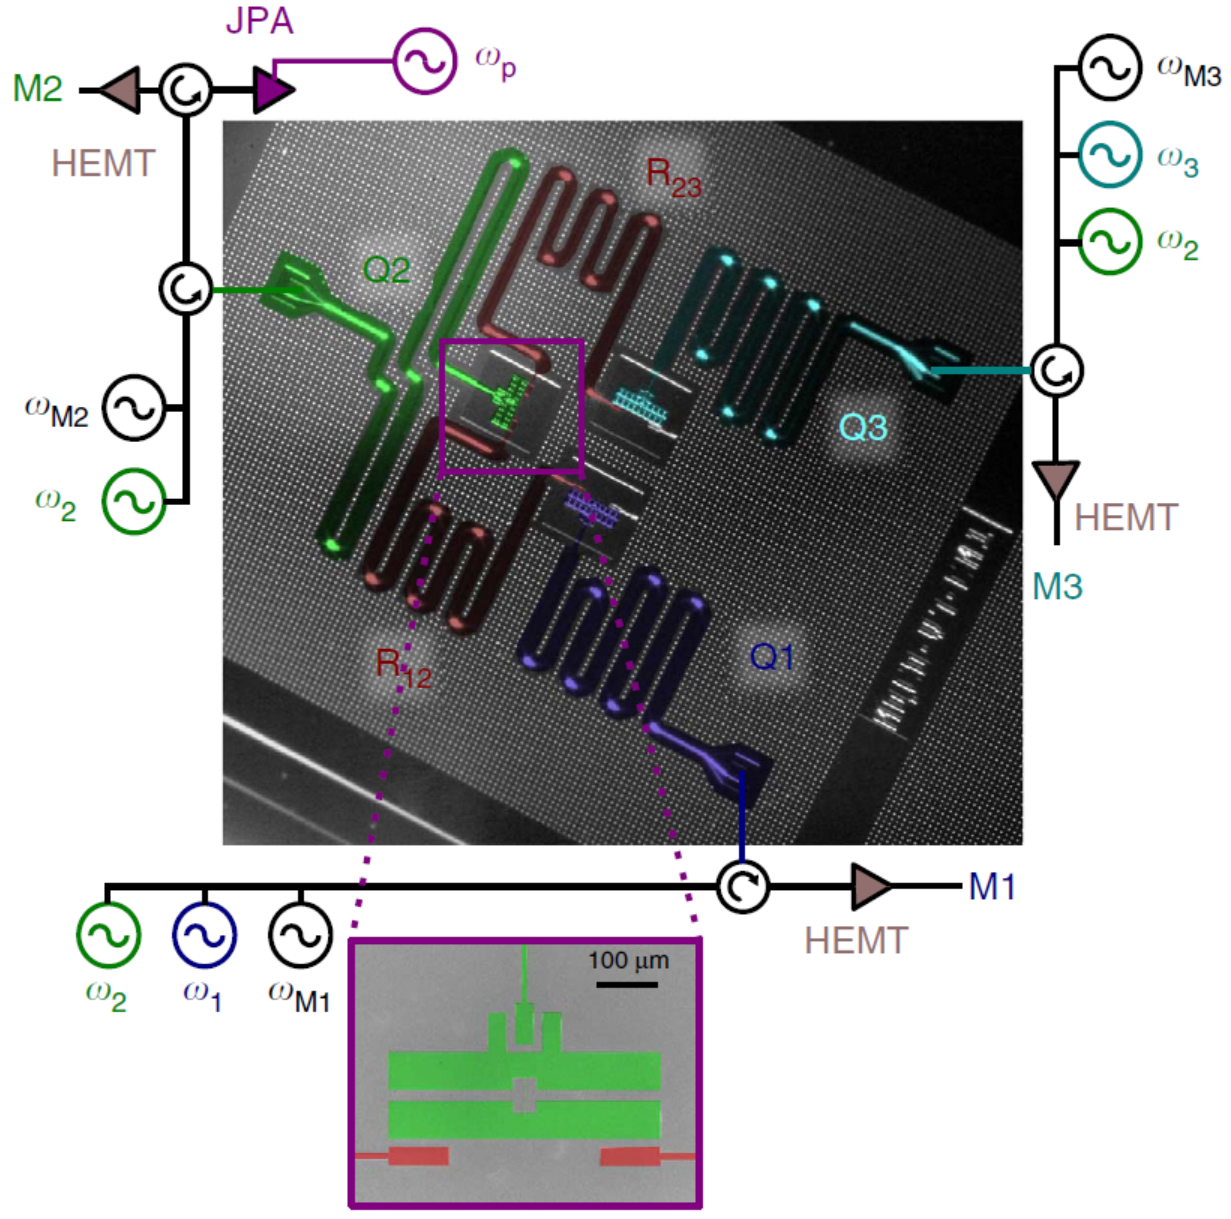
\includegraphics[width=4in]{review/IBMTransmon2014.png}
                \caption{The IBM transmon design. Adapted from Ref.~\onlinecite{Chow2014}.}
                \label{fig:IBMTransmon2014}
            \end{figure}


Another group at IBM adopted the 3D transmon design on 2D\cite{Chow2014,Takita2017} and was followed by other groups\cite{Mlynek2014,Pechal2016,Walter2017}. Based on their design, IBM initiated IBM Q in 2015 and provided a 5-qubit processor to public access\cite{IBMQ}. Recently they announced that they've successfully built and tested a 16-qubit processor for developers, researchers, and programmers via the IBM Cloud, and a 17-qubit prototype commercial processor\cite{IBM16QubitsOriginal}. Also recently a group in China showed a 10-qubit processor based on Xmon design\cite{Song2017}. D-Wave System Inc. announced quantum processors with hundreds of qubits\cite{Shin2014}, but those qubits have poor coherence properties and were not considered as a general quantum processor\cite{devoret2013superconducting}.



            \begin{figure}[h]
                \centering
                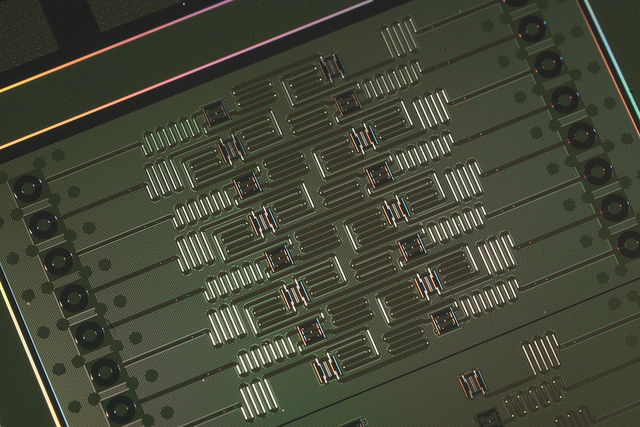
\includegraphics[width=4in]{review/ibmbuildsits.jpg}
                \caption{The IBM 16-qubit processor. Adapted from Ref.~\onlinecite{IBM16QubitsOriginal}.}
                \label{fig:ibmbuildsits}
            \end{figure}


After the increase in coherence time and the demonstration of basic algorithms and scalability, proposals and experiments turn to focus more on new architecture. One problem encountered when trying to scale up the superconducting qubit system is crossing of control, coupling and readout lines. Possible solutions require to go beyond the 2D structure, such as air bridge crossovers\cite{Versluis2016}, flip-chip\cite{Yorozu2006}, employing waveguide package resonance modes\cite{Minev2016} and using connected 3D cylindrical cavities\cite{Axline2016}. In addition, there are groups working on coupling superconducting qubits to flying qubits and mechanical resonators\cite{Palomaki2013,Reed2017,Keller2017}, aiming for the 6th and 7th DiVincenzo criteria.


% section history_of_the_development_of_transmon_qubit (end)


\section{Technical improvements} % (fold)
\label{sec:technical_improvements}

Much of the progress in the development of superconducting qubits came from clever design optimizations and technical improvements. The technical improvements can be roughly divided to several aspects including improving resonator quality factors, improving qubit control and measurement fidelity, and protecting qubits from decoherence.


Superconducting resonators were modeled and characterized in Ref.~\onlinecite{goppl2008coplanar}. The theoretic model was described in detail and agreements of frequencies and $Q$ factors between design and experiments were achieved. To increase the energy decay time, the major loss mechanism in CPW resonators were identified as surface two level systems (TLS)\cite{Gao2008Exp}. The quality factor measurement was further shown to agree with photon decay time  measurement by qubit-resonator swap experiments and surface TLS mechanism confirmed\cite{Wang2009}. The loss was shown to decrease by increasing the gap between the center conductor and the ground plane. Barends \etal{} increased the $Q$ factor up to $500\times 10^3$ by using NbTiN and removing dielectric materials from high electric field region\cite{Barends2010APL}. The surface loss simulation was carried out in Ref.~\onlinecite{Wenner2011Surface} and they found the dominant loss were from the metal-substrate and substrate-air interface. The same group of people soon made superconducting CPW resonators with $Q$ above $10^6$ by producing very smooth and clean aluminum layer and single crystal sapphire substrate\cite{Megrant2012}. The energy loss can also be reduced by reducing the participation rate of the dielectric materials, such as etching the substrate away from high electric fields\cite{Bruno2015}. As for 3D cavity, 10ms single photon lifetime at single photon level was achieved by Reagor \etal{}\cite{Reagor2013}. 3D cavities benefit from small participation ratio of the surfaces and hence the surface properties have smaller impact on the quality factors. The frequency shift in 3D cavities is also four orders smaller than in planar resonators when increasing temperature, but planar resonators have better scalability. There are detailed thesis about 2D\cite{Geerlings2013} and 3D\cite{Reagor2015thesis} resonator theory and design.


The basic qubit control methods were presented in Sec.~\ref{sub:control_and_readout_of_transmon_qubits}. However, actual qubits have other energy levels which lead to state leakage for non-ideal microwave pulse with finite frequency span, especially for transmon qubits with relatively weak nonlinearity. Motzoi \etal{} proposed an analytic approach they called Derivative Removal by Adiabatic
Gate (DRAG) to maximize gate fidelity\cite{Motzoi2009}. By using a second quadrature control approximately equal to the derivative of the first, they showed pulse envelopes agree with numeric optimization and demonstrated weak nonlinearity is sufficient for quantum gates. For two-qubit gates, the usual protocol\cite{DiCarlo2009} requires frequency tunability or uses ac Stark shift\cite{Majer2007} (also called resonator-induced PHASE gate). For fixed-frequency qubits with fixed linear coupling, an effective coupling can be induced by irradiating the control qubit at the transition frequency of the target qubit\cite{Rigetti2010}. For resonator-induced PHASE (RIP) gate, Cross \etal{} optimized the pulse shapes to reduce dephasing and decoherence, and to reduce the gate duration\cite{Cross2015}. They showed gates with infidelity $\sim 6\times 10^{-4}$ and gate time $\sim 120$ns. The RIP gate and controlled-Z gate are demonstrated with fixed-frequency qubits in Ref.~\onlinecite{Paik2016}. For characterizing the gate fidelity, randomized benchmarking was proposed by Kelly \etal{}\cite{Kelly2014}. As for qubit readout, most improvements came with improvements on amplifiers, such as Josephson bifurcation amplifier (JBA)\cite{Siddiqi2004} and Josephson parametric converter (JPC)\cite{Bergeal2010}. Ref.~\onlinecite{Sliwa2016} provides an inclusive introduction to JBA and JPC.




            \begin{figure}[h]
                \centering
                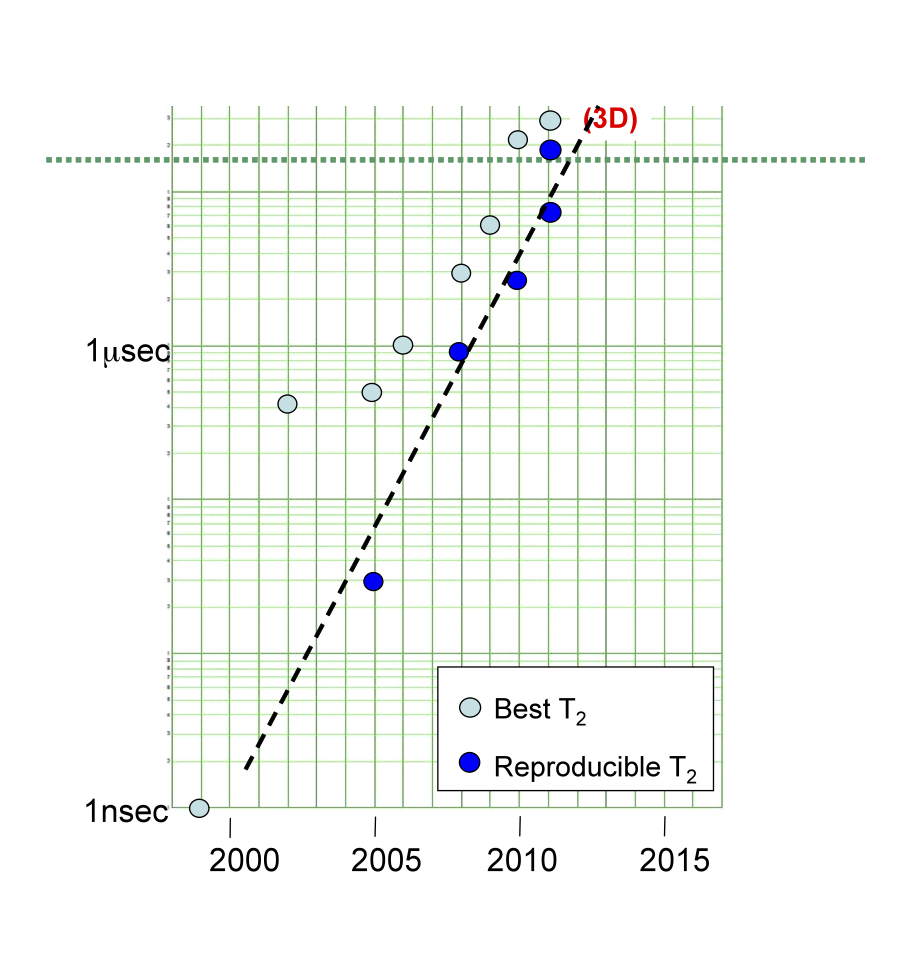
\includegraphics[width=3.5in]{review/SCQubitCoherence.png}
                \caption{The evolution of superconducting qubit $T_2$ time, where the dotted green line shows the necessary value for fault-tolerant quantum computing. Adapted from Ref.~\onlinecite{SteffenViewpoint}.}
                \label{fig:SCQubitCoherence}
            \end{figure}



The superconducting qubit coherence is steadily increasing as shown in Fig.~\ref{fig:SCQubitCoherence}. A lot of technical improvements were necessary to achieve such high coherence and Ref.~\onlinecite{Martinis2014Report} provides an extensive discussion on various decoherence sources and technical improvements. In summary, small junction is prefered to avoid defects. Removing loss from trapped vortices and quasiparticles by magnetic\cite{Barends2011,Martinis2014Report} and infrared\cite{Corcoles2011,Barends2011} shielding is required for reliable resonator $Q$ measurement and for higher qubit coherence. Other crucial technical improvements include effects of wirebond\cite{Wenner2011} and on-chip airbridge for eliminating slot-line modes\cite{Chen2014}. There are also groups trying to develop on-chip microwave circulator and isolator for quantum-limited performance\cite{Kerckhoff2015}.

% section technical_improvements (end)






\bibliographystyle{apsrev4-1}
\bibliography{refs}% Produces the bibliography via BibTeX.

\end{document}
%
% ****** End of file apssamp.tex ******



